\section{Hydrodynamics}
\mascaret solves the shallow water equations for incompressible flow, hydrostatic pressure and uniform distribution of velocities along the vertical axis. The flow slope and the horizontal curvature radius are supposed low. Wind effects on the free surface are also neglected. Flow is described on each section through mean velocity and mean free surface elevation.

\begin{CommentBlock}{Limit} 
	To use \courlis, only one reach can be considered. Besides, only the main channel can be taken into account and no singularities can be modeled.
\end{CommentBlock}

%%%%%%%%% ST VENANT %%%%%%%%%
\subsection{Shallow water equations}
The shallow water equations with variable section are given below :
\bequ
    \left\{
        \begin{array}{ll}
            \frac{\partial S}{\partial t} + \frac{\partial Q}{\partial x} = q_l\\
            \frac{\partial Q}{\partial t} + \frac{\partial \beta \frac{Q^2}{S}}{\partial x} + gZ\left( \frac{\partial Z}{\partial x} +J\right)= \frac{Q}{S} q_l\\
        \end{array}
    \right.
    \label{eq:shallow}
\eequ

with :
\begin{itemize}
	\item $S$ the wetted area ;
	\item $q_l$ the lateral inflows (confluence) in $m^2.s^{-1}$ ;
	\item $Q$ the mean discharge across the section ;
	\item $Z$ the free surface elevation ;
	\item $g$ the acceleration due to gravity ;
	\item $J$ the mean energy dissipation rate ;
	\item $\beta$ accounts for the variations of the real flow velocity accross the section \cite{mascaret_guide}.
\end{itemize}

\nomenclature{$S$}{Wetted area \nomunit{$m^2$}}
\nomenclature{$t$}{Time \nomunit{$s$}}
\nomenclature{$x$}{Longitudinal space variable \nomunit{$m$}}
\nomenclature{$q_l$}{Lateral inflows \nomunit{$m^2.s^{-1}$}}
\nomenclature{$g$}{Gravity acceleration \nomunit{$m^2.s^{-1}$}}
\nomenclature{$Q$}{Mean discharge accross the section \nomunit{$m^3.s^{-1}$}}
\nomenclature{$Z$}{Mean free surface elevation across the section \nomunit{$m$}}
\nomenclature{$J$}{Mean energy dissipation rate or energy slope \nomunit{$m.m^{-1}$}}

%%%%%%%%% RUGOSITE %%%%%%%%%
\subsection{Friction}
Bed and shores shear stress is taken into account through the Strickler friction law :
\bequ
	J = \frac{Q^2}{S^2 K^2 R_h^{\frac{4}{3}}}
	\label{eq:strickler}
\eequ
where :
\begin{itemize}
	\item $K$ is the Strickler coefficient ;
	\item $R_h$ the hydraulic radius.
\end{itemize}

The local shear stress $\tau_{tot}$ is computed by :

\bequ
	\tau_{tot} = \rho_w g R_h J = \frac{\rho_w g U^2}{K^2 R_h^{\frac{1}{3}}}
	\label{eq:contrainte_totale}
\eequ
For real cases, the hydraulic radius is usually approximated by the mean water depth across the section : $R_h \sim H$.
This option is activated by default in \courlis. 

\nomenclature{$H$}{Mean water depth across the section \nomunit{$m$}}
\nomenclature{$K$}{Strickler coefficient \nomunit{$m^{\frac{1}{3}}.s^{-1}$}}
\nomenclature{$R_h$}{Hydraulic radius \nomunit{$m$}}

%%%%%%%%% PLANIMETRAGE %%%%%%%%%
\subsection{Vertical discretization}
\label{planim}

Vertical discretization is used to transform cross-sections (2D) to unidimensional variables. Curves are generated for each section to link hydraulic radius, discharges, wetted areas, wetted perimeters and widths at the free surface to the elevation (starting at the lowest point of the section with a spatial step chosen by the user as shown on the Figure \ref{fig:planimetrage} below). 

\begin{figure}[htb!]
    \centering
    \includegraphics[width=\textwidth]{./graphics/planimetrage.png}
    \caption{Vertical discretization of a section : for each elevation, the width at the free surface and the middle point abscissa of the free surface are computed}
    \label{fig:planimetrage}
\end{figure}

For long-term simulations with a lot of bed evolutions, vertical discretization becomes time-consuming et can represent on its own up to more than 90\% of the total calculation time \cite{thesis_ung}. Clipping parameters can reduce the calls to the vertical discretization process. 

%%%%%%%%% TRANSPORT SOLIDE %%%%%%%%%
\section{Sediment transport}
\label{sediment_transport_th}
\courlis development was initiated in 1990 by EDF to model fine particles transport for the emptying of the Grangent reservoir in 1995. The bedload module of \courlis has been maintained and developed since 2012 and the Hydraulic Engineering Centre of EDF is officialy in charge of this module inside EDF since 2015.

The two modules can not be used simultaneously so no sediment mixing can be modeled with \courlis.

Up to 6 sediment layers (i.e. 7 interfaces) can be modeled in \courlis. Sediment interfaces are described in the geoC file (cf \S \ref{geoC_file}) and define homogeneous layers of sediment such as a 100$\%$ sand layer, a 100$\%$ silt layer and a mixed silt-sand sediment layer with the suspension module or a gravel layer and a bottom layer with the bedload module for example. Their elevation, and thus the width of the sediment layers, can vary transversaly as shown on Figure \ref{fig:layers} below.

\begin{figure}[htb!]
   \begin{minipage}[c]{.48\linewidth}
	\includegraphics[width=\textwidth]{./graphics/Plong.png} 
	\caption{Longitudinal profile of a reach}
	\label{fig:PLong}
   \end{minipage} \hfill
   \begin{minipage}[c]{.48\linewidth}
	\includegraphics[width=\textwidth]{./graphics/layers.png} 
	\caption{Cross-section view of sediment layers in \courlis}
	\label{fig:layers}
   \end{minipage}
\end{figure}

%\begin{figure}[htb!]
%    \centering
%    \includegraphics[width=0.7\textwidth]{./graphics/layers.png}
%    \caption{Sediment layers in \courlis}
%    \label{fig:layers}
%\end{figure}

The local shear stress can be decomposed into a stress associated to the skin friction, also called efficient shear stress, $\tau_{eff}$ and a stress due to bed forms $\tau_{forms}$ : 
$\tau_{tot} = \tau_{eff} + \tau_{forms} $
The skin friction coefficient is often computed from grain sizes, for example with the Strickler formula (Equation \ref{eq:strickler_kp}) or the Meyer-Peter and Müller formula (Equation \ref{eq:MPM_kp}).

\bequ
	K_p = \frac{21}{d_{50}}^\frac{1}{6}
	\label{eq:strickler_kp}
\eequ

\bequ
	K_p = \frac{26}{d_{90}}^\frac{1}{6}
	\label{eq:MPM_kp}
\eequ
$d_{50}$ is the median grain diameter and $d_{90}$ is the diameter for which 90\% of the grains are smaller.

\begin{WarningBlock}{Warning}
	For really fine sediment (< 200 $\mu m$ and cohesive sediment), these formulae become irrelevant and would give surfaces too smooth for natural beds. 
	In practice, skin friction should be limited to a maximal value of 85.
	This is the case when looking for deposition and erosion conditions for cohesive sediment ; a critical shear stress value of 85 Pa is systematically used.
\end{WarningBlock}

The efficient shear stress is estimated as 
\bequ
	\tau_{eff} = \tau_{tot} \left( \frac{K}{K_p} \right)^\gamma
\eequ  
with $\gamma$ a coefficient, by default equal to 2.

The Shields number $\theta$ is defined as :
\bequ
	\theta = \frac{\tau_{tot}}{(\rho_s-\rho_w) g d_{50}}
\eequ

Using Equation \ref{eq:contrainte_totale}, this expression becomes :
\bequ
	\theta = \frac{U^2}{R K^2 R_h^{\frac{1}{3}} d_{50}}
	\label{eq:shields}
\eequ
 $R$ is the relative reduced density $R=\frac{\rho_s}{\rho_w}-1 = s - 1$.

%%%%%%%%%%%%%%%%%%%%%%% SUSPENSION %%%%%%%%%%%%%%%%%%%%%%%
\subsection{\Csuspension}
Sediment in \Csuspension are considered as a passive tracer (no influence on the hydrodynamics), hence the fluid is always considered as a Newtonian fluid. 
The conservative form of the advection-diffusion equation for suspended sediment transport transport links the averaged concentration $C$ of the sediment with the erosion and deposition source terms $E$ and $D$.

\bequ
    \frac{\partial SC}{\partial t} + \frac{\partial QC }{\partial x}=\frac{\partial}{\partial x} \left (k_x S \frac{\partial C}{\partial x} \right) + E - D + q_{confluence}
\eequ

\begin{itemize}
	\item $k_x$ is the longitudinal dispersion coefficient ;
	\item $q_{confluence}$ the local inflows at a confluence for example.
\end{itemize}
The longitudinal dispersion coefficient can be estimated from \cite{Kas02} as done in \cite{Hau14}. 

Cohesive and non-cohesive sediment transport are supposed independant.

%%%%%%%%% VASE %%%%%%%%%
\subsubsection{Cohesive sediment fluxes}
%\tau_{tot} = \frac{\rho g H U^2}{K_p^2 R_h^{\frac{4}{3}}} ???
Cohesive sediment transport is considered unsaturated, i.e. concentration in the fluid is not limited (no saturation effect).
Deposition flux for cohesive sediment is computed with the empirical Krone law \cite{krone}.
\bequ
    \label{eq:krone}
    D = \left\{
        \begin{array}{ll}
            w_s C \left(1- \frac{\tau}{\tau_{c, deposition}}\right) \  \textrm{if}\  \tau < \tau_{c, deposition} , \\
            0 \  \textrm{otherwise}\\
        \end{array}
    \right.
\eequ
where $\tau$ is the bed shear stress, $\tau_{cr, deposition}$ the critical bed shear stress for deposition and $w_s$ the settling velocity for silts. 
 
Similarly, erosion flux is computed with the empirical Partheniades law \cite{partheniades} :

\bequ
    \label{eq:parth}
    E = \left\{
        \begin{array}{ll}
            M \left(\frac{\tau}{\tau_{c, erosion}} - 1 \right)  \  \textrm{if}\  \tau > \tau_{c, erosion} , \\
            0 \  \textrm{otherwise}\\
        \end{array}
    \right.
\eequ
where $\tau_{cr, erosion}$ is the critical bed shear stress for erosion and $M$ the Partheniades constant.
\begin{WarningBlock}{Note}
	For cohesive sediment, the critical bed shear stress $\tau_{cr}$ may be different for deposition and erosion, i.e. there can be a range of bed shear stresses for which there is no deposition or erosion (suspended load). 
	This is not the case for non-cohesive sediment. 
\end{WarningBlock}

%%%%%%%%% SAND %%%%%%%%%
\subsubsection{Non-cohesive sediment fluxes}
Sand transport is supposed saturated and is estimated via the Engelund-Hansen formula \cite{engelund}.
This formula is valid for grain sizes between 0.15 mm and 0.9 mm ($d_{50}$) and low slopes. 

\bequ
    \label{eq:engelund}
    q_s = 0.05 \sqrt{\frac{Rd_{50}^3}{g}} K^2 R_h^{\frac{1}{3}} \theta^{\frac{5}{2}}
\eequ
with $\theta$ the Shields number defined in Equation \ref{eq:shields}.

An equilibrium concentration is then defined as $C_{eq}=\frac{q_s \rho_s}{Q}$. 
When the solid discharge becomes higher than the transport capacity $C > C_{eq}$, the sediment flux becomes a deposition flux. Similarly, when the solid discharge is lower than the transport capacity $C < C_{eq}$, the flux becomes an erosion flux as described in the following equation :
\bequ
    q_s = \left\{
        \begin{array}{ll}
            \alpha w_s (C_{eq} - C)  \  \textrm{if}\  C > C_{eq} , \\
            \alpha w_s (C - C_{eq})  \  \textrm{otherwise}\\
        \end{array}
    \right.
\eequ
where $\alpha$ is an adjustment coefficient to the new equilibrium for suspension \cite{Che10}. 
It represents the velocity with which the sediment system tends to its new equilibrium state.
The sand settling velocity $w_s$ can be estimated thanks to the Stokes law (1851) or the Camenen formula \cite{Cam04}.


\nomenclature{$\alpha$}{Adjustment coefficient to the new equilibrium for suspension \nomunit{$\emptyset$}}

\nomenclature{$C$}{Suspended sediment concentration \nomunit{$g.L^{-1}$}}
\nomenclature{$I_f$}{Bottom slope \nomunit{$m/m$}}
\nomenclature{$I_{solid\ inflows}$}{Equilibrium slope for solid inflows \nomunit{$m/m$}}
\nomenclature{$k_x$}{Longitudinal dispersion coefficient along the $x$ axis \nomunit{$m^2.s^{-1}$}}
\nomenclature{$w_s$}{Settling velocity \nomunit{$m.s^{-1}$}}
\nomenclature{M}{Partheniades constant \nomunit{$kg.m^{-2}.s^{-1}$}}

%%%%%%%%% EVOLUTION DES FONDS %%%%%%%%%
\subsubsection{Bed evolution}

The bed evolution of the layer i during $\Delta t$ is computed with the solid discharges of deposition and erosion of the different layers :
\bequ
    \Delta h_{i, deposition}(\Delta t) = \frac{q_{deposition}\Delta t}{C_i}
\eequ

\bequ
    \Delta h_{i, erosion}(\Delta t)  = -\left(\sum h_{k, (\Delta t - \Delta t_1)} + \frac{q_{erosion}\Delta t_1 }{C_{i}}\right)
\eequ

where the variation in height of the layer $i$ by deposition or erosion is noted $\Delta h_i$ end the height of the layer $k$ eroded between $\Delta t_1$ and $\Delta t$ is noted $h_{k, (\Delta t - \Delta t_1)}$.

\nomenclature{$\Delta h_i$}{Height evolution of the sediment layer $i$ by deposition or erosion \nomunit{$m$}}
\nomenclature{$h_{i, \Delta t - \Delta t_1}$}{Height of the sediment layer $i$ eroded between $\Delta t_1$ and $\Delta t$ \nomunit{$m$}}

%%%%%%%%%%%%%%%%%%%%%%% BEDLOAD %%%%%%%%%%%%%%%%%%%%%%%
\subsection{\Cbedload}
For now, only one grain size distribution can be given to \Cbedload for all layers and all sections. 
\Cbedload is therefore commonly used with only one sediment layer i.e. two interfaces (one interface between the movable gravel bed and the water and a second one to separate the gravel bed from immovable non-erodible materials).
 
%%%%%%%%% EXNER %%%%%%%%%
\subsubsection{Bed evolution}
 This module is based on the Exner continuity equation (\ref{eq:exner}) to model gravel transport and bed evolutions in rivers or reservoirs. It does not take into account armoring and paving phenomena.

\bequ
     \rho_S (1-\rho) \frac{\partial Z_b}{\partial t} + \frac{\partial Q_s}{\partial x} = 0 
     \label{eq:exner}
\eequ

Resolution is done thanks to a finite volume scheme. The numerical flux term between two cells is computed with an uncentered scheme depending on the flow regime \cite{thesis_ung} : 

\begin{figure}[H]
	\centering
	\subfloat[Subcritical input -- Subcritical output]{
			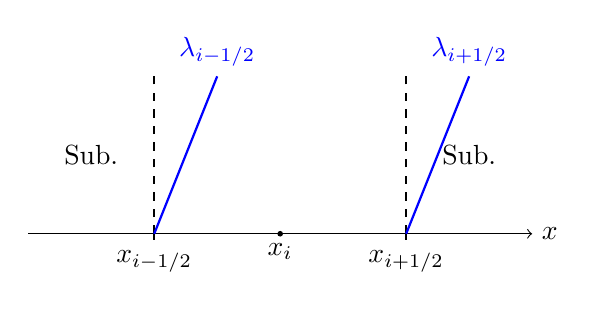
\begin{tikzpicture}[scale=0.4]
			  \draw[->]         (-8,0) -- (8,0)   node[right] {$x$};
			  \draw[thick,dashed]  (-4,0) -- (-4,5.);
			  \draw[thick,dashed] (4,0) -- (4,5.)  node[above] {};

			  \draw[thick] (-4,0.2)--(-4,-0.2) node[below] {$x_{i-1/2}$};
			  \draw[thick] (4,0.2)--(4,-0.2) node[below] {$x_{i+1/2}$};
			  \draw[fill=black] (0,0) circle (2pt) node[below]{$x_{i}$};

			  \draw (-6,2.5) node {Sub.};
			  \draw (6,2.5) node {Sub.};
			  \draw[color=blue, thick]  (-4,0) -- (-2,5)   node[above] {$\lambda_{i-1/2}$};
			  \draw[color=blue, thick]  (4,0) -- (6,5)     node[above] {$\lambda_{i+1/2}$};
			\end{tikzpicture}
	\label{fluvin_fluvout}
	}
	\hfill
	\subfloat[Supercritical input -- Supercritical output]{
		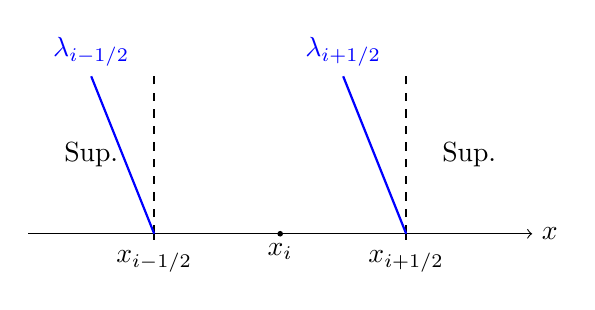
\begin{tikzpicture}[scale=0.4]
		  \draw[->]         (-8,0) -- (8,0)   node[right] {$x$};
		  \draw[thick,dashed]  (-4,0) -- (-4,5.);
		  \draw[thick,dashed] (4,0) -- (4,5.)  node[above] {};

		  \draw[thick] (-4,0.2)--(-4,-0.2) node[below] {$x_{i-1/2}$};
		  \draw[thick] (4,0.2)--(4,-0.2) node[below] {$x_{i+1/2}$};
		  \draw[fill=black] (0,0) circle (2pt) node[below]{$x_{i}$};

		  \draw (-6,2.5) node {Sup.};
		  \draw (6,2.5) node {Sup.};
		  \draw[color=blue, thick]  (-4,0) -- (-6,5)   node[above] {$\lambda_{i-1/2}$};
		  \draw[color=blue, thick]  (4,0) -- (2,5)     node[above] {$\lambda_{i+1/2}$};
		\end{tikzpicture}
		\label{torin_torout}
	}

	\subfloat[Subcritical input -- Supercritical output]{
		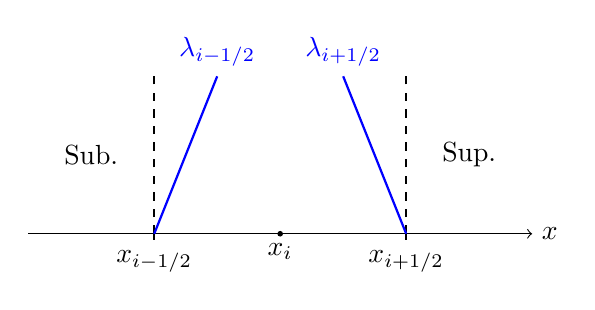
\begin{tikzpicture}[scale=0.4]
		  \draw[->]         (-8,0) -- (8,0)   node[right] {$x$};
		  \draw[thick,dashed]  (-4,0) -- (-4,5.);
		  \draw[thick,dashed] (4,0) -- (4,5.)  node[above] {};

		  \draw[thick] (-4,0.2)--(-4,-0.2) node[below] {$x_{i-1/2}$};
		  \draw[thick] (4,0.2)--(4,-0.2) node[below] {$x_{i+1/2}$};
		  \draw[fill=black] (0,0) circle (2pt) node[below]{$x_{i}$};

		  \draw (-6,2.5) node {Sub.};
		  \draw (6,2.5) node {Sup.};
		  \draw[color=blue, thick]  (-4,0) -- (-2,5)   node[above] {$\lambda_{i-1/2}$};
		  \draw[color=blue, thick]  (4,0) -- (2,5)     node[above] {$\lambda_{i+1/2}$};
		\end{tikzpicture}
		\label{fluvin_torout}
	}
	\hfill
	\subfloat[Supercritical input -- Subcritical output]{
		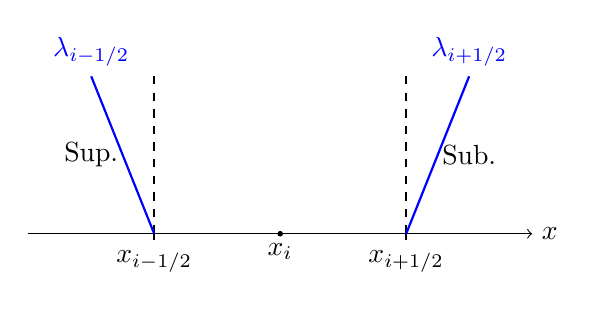
\begin{tikzpicture}[scale=0.4]
		  \draw[->]         (-8,0) -- (8,0)   node[right] {$x$};
		  \draw[thick,dashed]  (-4,0) -- (-4,5.);
		  \draw[thick,dashed] (4,0) -- (4,5.)  node[above] {};

		  \draw[thick] (-4,0.2)--(-4,-0.2) node[below] {$x_{i-1/2}$};
		  \draw[thick] (4,0.2)--(4,-0.2) node[below] {$x_{i+1/2}$};
		  \draw[fill=black] (0,0) circle (2pt) node[below]{$x_{i}$};

		  \draw (-6,2.5) node {Sup.};
		  \draw (6,2.5) node {Sub.};
		  \draw[color=blue, thick]  (-4,0) -- (-6,5)   node[above] {$\lambda_{i-1/2}$};
		  \draw[color=blue, thick]  (4,0) -- (6,5)     node[above] {$\lambda_{i+1/2}$};
		\end{tikzpicture}
		\label{torin_fluvout}
		}
	
	\caption{Different situations depending on the nature of the flow at the input and output of a cell from \cite{thesis_ung} - $\lambda$ is the wave velocity associated to the bed evolution.}
	\label{fig:allregcell}
\end{figure}

\nomenclature{$\lambda_i$}{Wave velocity associated to bed evolution in cell $i$ \nomunit{$m.s^{-1}$}}

Depending on the flow motion at the input and the output of the cell $i$, the variation of volume in the cell $i$ between two consecutive timsteps is computed from the following finite volume scheme :

\bequ
\begin{gathered}\label{eq:exner-scheme}
{(V)_i^{n+1} - (V)_i^n =}\\
\left\{
        \begin{array}{ll}
		  -\frac{\delta t}{\delta x} \left( (Q_s)_{i+1}^n - (Q_s)_{i}^n \right) & \textrm{if} \  (F_r)_{i-1/2} < 1 \  \textrm{and} \  (F_r)_{i+1/2} < 1 \  \textrm{(case \ref{fluvin_fluvout}),} \\
		  -\frac{\delta t}{\delta x} \left( (Q_s)_{i}^n - (Q_s)_{i-1}^n \right) & \textrm{if} \ (F_r)_{i-1/2} > 1 \  \textrm{and} \ (F_r)_{i+1/2} > 1 \  \textrm{(case \ref{torin_torout}),} \\
		  -\frac{\delta t}{2 \delta x} \left( (Q_s)_{i+1}^n - (Q_s)_{i-1}^n \right) & \textrm{if} \  (F_r)_{i-1/2} < 1 \  \textrm{and} \ (F_r)_{i+1/2} > 1 \  \textrm{(case \ref{fluvin_torout}),} \\
  0 & \textrm{if} \  (F_r)_{i-1/2} > 1 \  \textrm{and} \  (F_r)_{i+1/2} < 1 \  \textrm{(case \ref{torin_fluvout}).}
	\end{array}
	\right.
\end{gathered}
\eequ
where 
\begin{itemize}
	\item $(V)_i^n$ is the volume of sediment in the cell $i$ at the timestep $n$ ;
	\item $\delta t$ is the timestep ;
	\item $\delta x$ is the spacestep ;
	\item $(Q_s)_{i}^n$ is the solid discharge in the cell $i$ at the timestep $n$ given by the transport law ;
	\item $F_r$ is the Froude number defined such as \[ F_r = \dfrac{u}{\sqrt{gh_w}} \] with $h_w$ the water depth. 
\end{itemize}

\nomenclature{$h_w$}{Water depth \nomunit{$m$}}
\nomenclature{$F_r$}{Froude number \nomunit{$\emptyset$}}
\nomenclature{$V_i^n$ }{Volume of sediment in cell $i$ at the timestep $n$ \nomunit{$m^{3}$}}

The bottom elevation is then updated accordingly to the variation of volume computed above. The solid discharge $(Q_s)_{i}^n$ in cell $i$ at the timstep $n$ is computed with different transport formulae described below. 

\nomenclature{$Z_b$}{Bottom elevation \nomunit{$m$}}

Evolution of the river bottom is not applied in the same way for erosion and for deposition :
\begin{itemize}
 \item Evolution due to erosion is applied uniformely on all points of the river bottom located under the free surface ;
 \item Evolution due to deposition is applied horizontally (at constant elevation). For each horizontal deposition surface, the corresponding elevation is computed by linear interpolation of the curves generated by vertical discretization (cf Section \ref{planim}).
\end{itemize}

\begin{figure}[htb!]
    \centering
    \includegraphics[width=0.45\textwidth]{./graphics/erosion_deposition.png}
    \caption{Deposition and erosion mechanisms in \Cbedload}
    \label{fig:depo_ero}
\end{figure}

%%%%%%%%% FORMULES DE TRANSPORT %%%%%%%%%
\subsubsection{Transport formulae for the solid discharge}

Several transport formulae (cf Appendix \ref{app:formules_transport} for detailed expressions of these formulae) are available in \Cbedload :
\begin{itemize}
	\item Meyer-Peter and Müller (1948) \cite{MPM} : most commom transport formula, it is based on grain mouvement threshold concept and is valid for sediment sizes between 0.4 and \mbox{29 mm} and slopes between 0.4 and 2.4 \% \cite{lois_validite_recking}. This formula is not adapted to sand transport and is well known to underestimate solid transport at low flow rates. 
	\item Lefort (2015) : Lefort \cite{lefort} law was recently developed and validated over around 1 000 fields data and 3 400 laboratoy data. It is especially fitted for alpine rivers. This formula is valid for a wide range of slopes $I_f < 20\%$ and grain sizes $0.1\ mm < d_{50} < 55\ mm$. It was shown that this law remained relevant even with very high flow up to 28 000 m$^3/s$ \cite{lois_validite_recking}. This formula uses discharge which is easier to measure than bottom shear stress and therefore often offers a better estimation of transport rate. This formula is particularly suitable for gravel rivers but remains questionable for low flow.
	\item Recking (2013) \cite{recking2013} : This threshold formula was validated over 15 different reaches. This law is valid for grain sizes between 0.4 mm and 220 mm and a wide range of slopes $0.1\% < I_f < 7\%$\cite{lois_validite_recking}. It is especially suitable for gravel beds. 
	\item Recking (2015) \cite{recking2015}: In 2015, changes were proposed from the Recking formula to better take into account the effect of river morphologies on solid transport. The new formula was developped studying bedload measured in flumes (more than 12 data sets) and in the field (more than 133 data sets) \cite{recking2015}. 
\end{itemize}

%%%%%%%%%%%%%%%%%%%%%%% Slope stability %%%%%%%%%%%%%%%%%%%%%%%
\subsection{Slope stability}
\label{talus_th}

When emptying reservoirs, non-negligeable amount of sediment comes from sediment slide. Consequently, a simple sediment slide model was proposed in \courlis. It is available with both transport modules.

Slope stability is defined by two equilibrium slopes, one for underwater sediment $I_{stab, UN}$ and a second one for emerged sediment $I_{stab, EM}$.

\begin{CommentBlock}{Limit}
	Equilibrium slopes are given by the user but \courlis allows for only one value of ($I_{stab, UN}$, $I_{stab, EM}$) along the reach and for all sediment layers.
\end{CommentBlock}

Equilibrium slopes can be estimated thanks to soil measurements and empirical formulae proposed by Migniot \cite{Mig89} :
\bequ
	\tan I_{stab, UN} = k \tau_y
	\label{eq:stabUN}
\eequ

\bequ
	\tan I_{stab, EM} = k' \tau_y
	\label{eq:stabEM}
\eequ

where
\begin{itemize}
	\item $\tau_y$ is the intial stiffness of deposition;
	\item $k=0.01$ ;
	\item $k'=0.003$.
\end{itemize}

In all cross-section points, sediment slope is compared to the corresponding stability slope. If the sediment slope is larger than the stability slope, sediment crumbles to match the stability slope on this point.
Emerged sediment slide model is particularly relevant when emptying reservoirs as described above. On the other side, underwater sediment slide is essential to stabilize bed evolutions due to erosion. Indeed, \courlis can not reproduce channel enlargement, during flood for example, as free surface elevation and energy slope are supposed constant over the cross-section. Local shear stress is therefore maximal at the lower point where water depth is maximal and cause excessive erosion at the lower point and high lateral slopes as shown below on Figure \ref{fig:no_stab_model}. 

\begin{figure}[htb!]
	\centering
	\includegraphics[width=0.7\textwidth]{./graphics/chenal.png}
	\caption{Channel erosion with \courlis without slope stability model}
	\label{fig:no_stab_model}
\end{figure}

This model, based on a single threshold, remains simple and can still be improved. 

\begin{WarningBlock}{Warning}
	The user should also be aware that initial states can be unstable (initial geometry slopes higher than the stability slope) and therefore generate high, non-physical, sediment transport rates at the beginning of the simulation (mainly with \Csuspension). 
\end{WarningBlock}
%%%%%%%%%%%%%%%%%%%%%%% Coupling %%%%%%%%%%%%%%%%%%%%%%%
\subsection{Coupling between \courlis and \mascaret}
\label{coupling}
\begin{figure}[hbt!]
	\centering
	\includegraphics[width=\textwidth]{./graphics/coupling.png}
	\caption{Coupling between \courlis and \mascaret over a time $\Delta t = p \delta t_S = n \delta t_H$}
	\label{fig:coupling}
\end{figure}

The coupling between \courlis and \mascaret is weak. 
Shallow water equations are solved independently by the \mascaret kernel during $n$ timesteps. Hydraulics variables are used by \courlis for solid transport calculations and bed evolutions are given back to \mascaret after $p$ timesteps. Each code uses its own timestep $\delta t_H$ and $\delta t_S$. The hydraulics timestep $\delta t_H$ is chosen by the user while the solid transport timestep $\delta t_S$ is set such as :
$\Delta t = p \delta t_S = n \delta t_H$
The coupling parameters $p$ and $n$ are chosen by the user according to bed evolutions magnitude and speed. 

When the transcritical kernel of \mascaret (also called MASCARET) is used, the hydraulics timestep $\delta t_H$ can vary to match a Courant-Friedrich-Levy number set by the user (traditionally $CFL = 0.8$). 
This Courant-Friedrich-Levy number can reduce computational time as it adapts the hydraulics timestep to spacestep and hydraulics variables values at each iteration:
\bequ
	CFL = \left(  U+\sqrt{gH} \right)  \frac{\delta t_H}{\delta x}
	\label{eq:CFL}
\eequ
In this case, the sediment transport timestep $\delta t_S$ also varies during simulation accordingly. 

\nomenclature{$\delta t_H$}{Hydraulics timestep \nomunit{$s$}}
\nomenclature{$\delta t_S$}{Sediment transport timestep \nomunit{$s$}}



